% directive: erasureCodeSchemeFigure
% aria-label: Erasure code: the sender encodes a message M in Sigma^k into the chunks (j, Encode(M, j)) for j = 0 to N-1; some chunks are lost; the receiver decodes the set L of received chunks, which holds at least k chunks with distinct indices, and recovers M.
\documentclass[tikz,border=6pt]{standalone}
\usepackage[T1]{fontenc}
\usepackage{amsmath,amssymb}
\renewcommand{\familydefault}{\sfdefault}
\usepackage[eulergreek]{sansmath}
\sansmath
\usepackage{xcolor}
\usepackage{tikz}
\usetikzlibrary{positioning,calc,arrows.meta,fit,backgrounds,decorations.pathreplacing}
\definecolor{commentcolor}{HTML}{666666}
\definecolor{signalblue}{HTML}{3A76F0}
\definecolor{signalgreen}{HTML}{2A7B7B}
\definecolor{signalolive}{HTML}{4E7F60}
\definecolor{signalpurple}{HTML}{6B3FA0}
\definecolor{adversaryred}{HTML}{B42318}
\newcommand{\Encode}{\mathsf{Encode}}
\newcommand{\Decode}{\mathsf{Decode}}
\tikzset{
  panel/.style={draw=gray!45, line width=0.5pt, rounded corners=4pt, fill=gray!3, inner sep=6pt},
  algbox/.style={draw=signalolive!80, line width=0.7pt, rounded corners=3pt, fill=signalolive!10,
    inner sep=6pt, font=\small\sffamily, align=center},
  statebox/.style={draw=signalblue!70, line width=0.65pt, rounded corners=4pt, fill=signalblue!6,
    inner sep=6pt, font=\small\sffamily, align=center},
  keypill/.style={draw=signalpurple!75, line width=0.6pt, rounded corners=7pt, fill=signalpurple!9,
    inner xsep=8pt, inner ysep=4pt, font=\small\sffamily},
  chunk/.style={draw=signalblue!75, line width=0.55pt, rounded corners=2pt, fill=signalblue!9,
    minimum width=0.62cm, minimum height=0.50cm, inner sep=1pt, font=\scriptsize\sffamily},
  chunklost/.style={chunk, draw=gray!45, fill=gray!10, text=gray!55},
  sourcechunk/.style={chunk, draw=signalpurple!70, fill=signalpurple!9},
  goodpill/.style={draw=signalgreen!80, line width=0.65pt, rounded corners=7pt, fill=signalgreen!9,
    inner xsep=8pt, inner ysep=4pt, font=\small\sffamily},
  failpill/.style={draw=adversaryred!75, line width=0.65pt, rounded corners=7pt, fill=adversaryred!7,
    inner xsep=8pt, inner ysep=4pt, font=\small\sffamily},
  flow/.style={->, >=Stealth, line width=0.8pt, black},
  lossy/.style={->, >=Stealth, line width=0.5pt, gray!55, dashed},
  slot/.style={draw=gray!60, line width=0.5pt, minimum width=0.42cm, minimum height=0.42cm, inner sep=0pt},
  slotfull/.style={slot, fill=signalgreen!25, draw=signalgreen!70},
  slotempty/.style={slot, fill=white},
  lbl/.style={font=\small\sffamily, inner sep=2pt},
  slbl/.style={font=\scriptsize\sffamily, inner sep=1.5pt},
  note/.style={font=\scriptsize\sffamily\itshape, text=commentcolor, inner sep=1.5pt},
  theorybox/.style={draw=signalgreen!80, line width=0.8pt, rounded corners=4pt, fill=signalgreen!8,
    inner sep=7pt, font=\small\sffamily, align=center},
  instancebox/.style={draw=signalblue!70, line width=0.7pt, rounded corners=4pt, fill=signalblue!6,
    inner sep=7pt, font=\small\sffamily, align=center},
  instof/.style={->, >=Stealth, line width=0.8pt, black},
  uses/.style={->, >=Stealth, line width=0.7pt, dashed, signalolive},
  ecbox/.style={draw=signalblue!70, line width=0.7pt, rounded corners=3pt, fill=signalblue!7,
    inner sep=6pt, font=\small\sffamily, align=center},
  rolepill/.style={fill=signalgreen, text=white, rounded corners=5pt, inner xsep=9pt, inner ysep=4pt,
    font=\sffamily\bfseries},
  advpill/.style={draw=adversaryred!80, line width=0.7pt, rounded corners=5pt, fill=adversaryred!7,
    text=adversaryred, minimum width=1.05cm, minimum height=0.68cm, inner sep=3pt, font=\normalsize},
  timeline/.style={-, line width=0.6pt, gray!55},
}
\newcommand{\tagsf}[1]{{\scriptsize\sffamily\itshape\textcolor{commentcolor}{#1}}}
\newcommand{\notesf}[1]{{\scriptsize\sffamily\itshape\textcolor{signalpurple}{#1}}}

\begin{document}
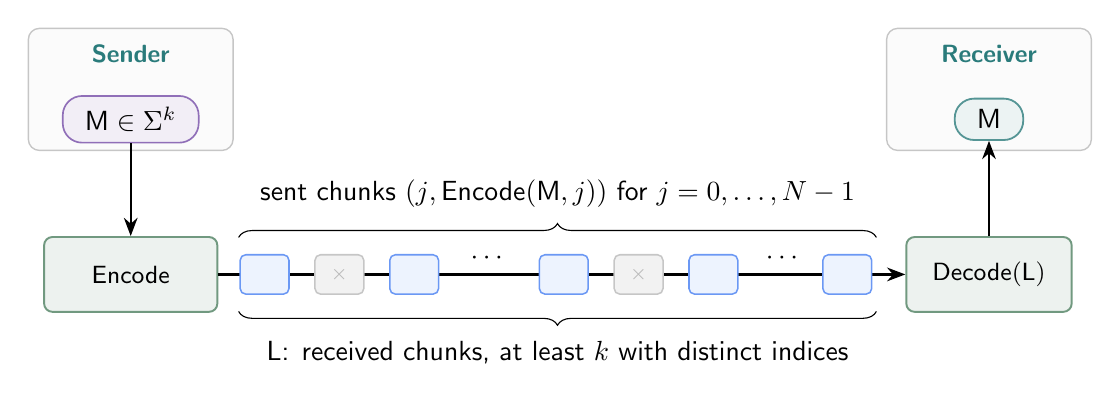
\begin{tikzpicture}[x=1cm,y=1cm]
  \node[panel, minimum width=2.6cm, minimum height=1.55cm] at (-5.45,1.10) (senderbox) {};
  \node[font=\small\sffamily\bfseries, text=signalgreen] at (-5.45,1.55) {Sender};
  \node[keypill, font=\normalsize] at (-5.45,0.72) (msgin) {$\mathsf M\in\Sigma^k$};
  \node[algbox, minimum width=2.20cm, minimum height=0.95cm] at (-5.45,-1.25) (enc) {$\Encode$};
  \draw[flow] (msgin.south) -- (enc.north);
  \node[algbox, minimum width=2.10cm, minimum height=0.95cm] at (5.45,-1.25) (dec) {$\Decode(\mathsf L)$};
  \draw[flow] (enc.east) -- (dec.west);
  \node[chunk] at (-3.75,-1.25) {};
  \node[chunklost] at (-2.80,-1.25) {$\times$};
  \node[chunk] at (-1.85,-1.25) {};
  \node[font=\normalsize] at (-0.90,-1.05) {$\cdots$};
  \node[chunk] at (0.05,-1.25) {};
  \node[chunklost] at (1.00,-1.25) {$\times$};
  \node[chunk] at (1.95,-1.25) {};
  \node[font=\normalsize] at (2.85,-1.05) {$\cdots$};
  \node[chunk] at (3.65,-1.25) {};
  \draw[decorate, decoration={brace, amplitude=5pt}] (-4.08,-0.78) -- (4.02,-0.78);
  \node[anchor=south, font=\normalsize\sffamily] at (-0.03,-0.52)
    {sent chunks $(j,\Encode(\mathsf M,j))$ for $j=0,\ldots,N-1$};
  \draw[decorate, decoration={brace, mirror, amplitude=5pt}] (-4.08,-1.72) -- (4.02,-1.72);
  \node[anchor=north, font=\normalsize\sffamily] at (-0.03,-1.98)
    {$\mathsf L$: received chunks, at least $k$ with distinct indices};
  \node[panel, minimum width=2.6cm, minimum height=1.55cm] at (5.45,1.10) (receiverbox) {};
  \node[font=\small\sffamily\bfseries, text=signalgreen] at (5.45,1.55) {Receiver};
  \node[goodpill, font=\normalsize] at (5.45,0.72) (msgout) {$\mathsf M$};
  \draw[flow] (dec.north) -- (msgout.south);
\end{tikzpicture}
\end{document}
